\section{一阶方法}
\label{sec:mfo-first-order}

三种几何运算齐备后，先看只用一阶信息的方法。于是要问：负切向梯度加回缩为什么能下降，步长如何选择，以及搬运历史方向怎样加快收敛又带来了哪些新的检查项？

\subsection{黎曼梯度下降}
\label{sec:mfo-rgd}

\paragraph{主要思想}
\term{黎曼梯度下降}（Riemannian gradient descent）在当前切空间中沿负梯度取步，再用回缩回到流形：
\begin{equation}
 \bm{x}^{(t+1)}=R_{\bm{x}^{(t)}}\bigl(-\alpha^{(t)}\bm{g}^{(t)}\bigr),\qquad\bm{g}^{(t)}=\operatorname{grad}f(\bm{x}^{(t)}).
 \label{eq:mfo-rgd}
\end{equation}

为什么这一步能下降？记$\phi(\alpha)=\hat{f}_{\bm{x}}(-\alpha\bm{g})$，这是一个普通的一元函数。由式~\eqref{eq:mfo-pullback-grad}，
\[
 \phi'(0)=\langle\operatorname{grad}f(\bm{x}),-\bm{g}\rangle=-\lVert\bm{g}\rVert_2^2<0.
\]
所以只要$\bm{g}\neq\bm{0}$，足够小的步长一定使目标下降。这个结论只用了回缩的一阶一致性，不需要二阶回缩。

步长的选择与欧氏情形完全平行，只是把比较对象换成拉回函数。Armijo条件要求
\begin{equation}
 f\bigl(R_{\bm{x}}(-\alpha\bm{g})\bigr)\leq f(\bm{x})-c_1\alpha\lVert\bm{g}\rVert_2^2.
 \label{eq:mfo-armijo}
\end{equation}
下降的检验必须针对回缩后的点，切平面上的点$\bm{x}-\alpha\bm{g}$根本不可行，其函数值没有意义。

\needspace{6\baselineskip}
\paragraph{变量}
\begin{itemize}
 \item $\bm{x}^{(t)}\in\mathbb{R}^3$：球面上的当前点，长度为一。
 \item $q^{(t)}$：Rayleigh商的取值，标量。
 \item $\bm{g}^{(t)}$：黎曼梯度，与$\bm{x}^{(t)}$垂直的三维向量。
 \item $\alpha$：当前试探步长；$c_1=\tfrac14$是Armijo常数，缩减因子取$\tfrac12$。
\end{itemize}

\paragraph{初始化}
取$\bm{x}^{(0)}$，初始试探步长$\alpha_0=1$，停止容差$\lVert\bm{g}^{(t)}\rVert_2\leq10^{-6}$。例中$\bm{x}^{(0)}=\tfrac13(2,2,1)^\top$，$f(\bm{x}^{(0)})=\tfrac89$。

\needspace{6\baselineskip}
\paragraph{每轮更新}
\begin{enumerate}
 \item 由式~\eqref{eq:mfo-rayleigh-grad}算$\bm{g}^{(t)}$。例中第$0$轮已算得
 \[
  \bm{g}^{(0)}=\frac{1}{27}(-14,4,20)^\top,\qquad\lVert\bm{g}^{(0)}\rVert_2^2=\frac{68}{81}.
 \]

 \item 令$\alpha=\alpha_0$，按式~\eqref{eq:mfo-sphere-retraction}算试探点，并检验式~\eqref{eq:mfo-armijo}，不满足时$\alpha$减半。例中第$0$轮先试$\alpha=1$：
 \[
  \bm{x}^{(0)}-\bm{g}^{(0)}=\frac{1}{27}(32,14,-11)^\top.
 \]
 归一化后的点是$(0.8738,0.3823,-0.3004)^\top$，目标值$0.7084$，下降$0.1805$，低于要求的$\tfrac14\cdot\tfrac{68}{81}\approx0.2099$，拒绝。

 \item 例中减半后试$\alpha=\tfrac12$，得到
 \[
  \bm{x}^{(0)}-\tfrac12\bm{g}^{(0)}=\frac{1}{27}(25,16,-1)^\top.
 \]
 由勾股定理，长度的平方是$1+\tfrac14\cdot\tfrac{68}{81}=\tfrac{98}{81}$，长度是$\tfrac{7\sqrt2}{9}$。

 \item 接受时令$\bm{x}^{(t+1)}$为该试探点。例中
 \[
  \bm{x}^{(1)}=\frac{(25,16,-1)^\top}{21\sqrt2}\approx(0.8418,0.5388,-0.0337)^\top.
 \]
 目标值$0.6468$，下降$0.2421$，超过要求的$0.1049$，接受。
\end{enumerate}

图~\ref{fig:mfo-rgd-step}画出这一轮的几何：两个候选点都在切平面上，沿径向回到球面后才可以比较。

\begin{BookInlineFigure}
 \centering
 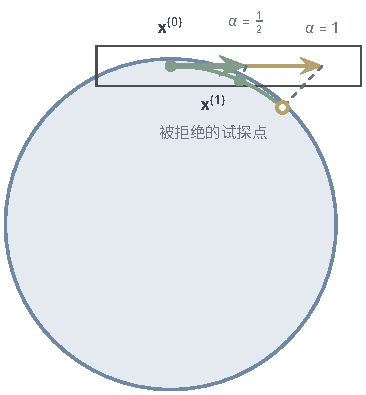
\includegraphics[width=62.0mm]{figures/05-optimization/06-constrained-optimization/tikz/mfo-rgd-step/figure.pdf}
 \caption{第$0$轮迭代的几何，视线接近垂直于$\bm{x}^{(0)}$与$\bm{g}^{(0)}$所在的平面。方框是切平面的一块，黄箭头和绿箭头分别是$\alpha=1$和$\alpha=\tfrac12$的切向步，虚线是归一化回缩。空心点未通过Armijo检验，绿点$\bm{x}^{(1)}$通过。}
 \label{fig:mfo-rgd-step}
\end{BookInlineFigure}

第$1$轮算得
\[
 \bm{g}^{(1)}\approx(-0.2472,0.3805,-0.0911)^\top,\qquad\lVert\bm{g}^{(1)}\rVert_2^2\approx0.2142.
\]
$\alpha=1$的试探点是$(0.9883,0.1436,0.0521)^\top$，目标值$0.5144$，下降$0.1324$，超过要求的$0.0536$，接受。

第$2$轮$\lVert\bm{g}^{(2)}\rVert_2^2\approx0.0443$。$\alpha=1$的试探点目标值$0.5152$，反而上升，拒绝；$\alpha=\tfrac12$的试探点目标值$0.5036$，下降$0.0107$，超过要求的$0.0055$，接受。表~\ref{tab:mfo-rgd-run}汇总前几轮。

\begin{BookInlineTable}
 \centering
 \caption{贯穿例的黎曼梯度下降，回溯线搜索。}
 \label{tab:mfo-rgd-run}
 \begin{tabular}{lllll}
  \toprule
  $t$ & $\bm{x}^{(t)}$ & $f(\bm{x}^{(t)})$ & $\lVert\bm{g}^{(t)}\rVert_2$ & 接受的$\alpha$\\
  \midrule
  $0$ & $(0.6667,0.6667,0.3333)$ & $0.8889$ & $0.9162$ & $0.5$\\
  $1$ & $(0.8418,0.5388,-0.0337)$ & $0.6468$ & $0.4628$ & $1$\\
  $2$ & $(0.9883,0.1436,0.0521)$ & $0.5144$ & $0.2104$ & $0.5$\\
  $3$ & $(0.9970,0.0735,-0.0252)$ & $0.5036$ & $0.1051$ & $0.5$\\
  $4$ & $(0.9992,0.0369,0.0125)$ & $0.5009$ & $0.0526$ & $0.5$\\
  \bottomrule
 \end{tabular}
\end{BookInlineTable}

末尾几轮梯度范数每轮减半。这有明确的来由：$\bm{e}_1$处切向曲率是$1$和$3$，局部迭代相当于$\bm{v}\mapsto(\bm{I}-\alpha\bm{H})\bm{v}$，$\alpha=\tfrac12$时两个因子是$\tfrac12$和$-\tfrac12$。这也解释了第三个坐标的符号交替。当$\lVert\bm{g}^{(t)}\rVert_2\leq10^{-6}$时停止，最终得到$\bm{x}^{(T)}\approx\bm{e}_1$。

图~\ref{fig:mfo-rgd-path}是球面上的路径，图~\ref{fig:mfo-rgd-convergence}是收敛曲线。固定步长$\alpha=\tfrac29$的路径更平缓，但每轮的收缩因子是$1-\tfrac29=\tfrac79$，慢得多。

\begin{BookInlineFigure}
 \centering
 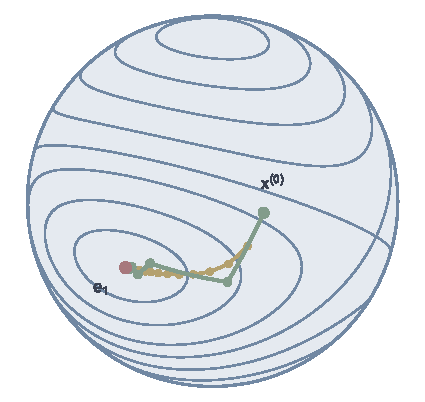
\includegraphics[width=72.0mm]{figures/05-optimization/06-constrained-optimization/matplotlib/mfo-rgd-path/figure.pdf}
 \caption{球面上的迭代路径，蓝线是目标的等高线。绿色为回溯线搜索（$c_1=\tfrac14$），黄色为固定步长$\alpha=\tfrac29$，点之间用大圆弧连接，红点是极小点。}
 \label{fig:mfo-rgd-path}
\end{BookInlineFigure}

\begin{BookInlineFigure}
 \centering
 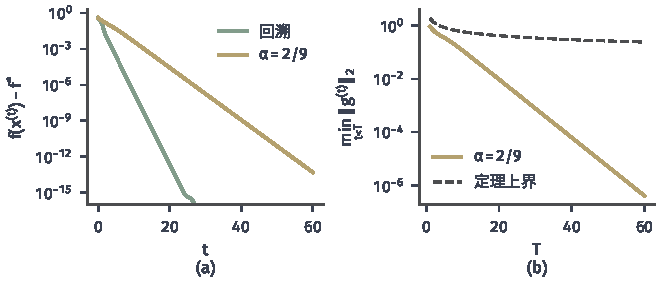
\includegraphics[width=112.0mm]{figures/05-optimization/06-constrained-optimization/matplotlib/mfo-rgd-convergence/figure.pdf}
 \caption{贯穿例上的收敛。(a)~目标误差，绿色回溯，黄色固定步长$\tfrac29$。(b)~固定步长下至第$T$轮为止的最小梯度范数（黄）与定理~\ref{thm:mfo-rgd-rate}给出的上界（灰虚线，$L=\tfrac92$）。上界有效，但对这个问题偏松。}
 \label{fig:mfo-rgd-convergence}
\end{BookInlineFigure}

\paragraph{收敛性}
欧氏分析的关键是下降引理，流形上只需要把它改写成对拉回函数的假设。这个假设是下面的上界，称为拉回的$L$光滑性：对所考虑的$\bm{x}$和$\bm{v}$，
\begin{equation}
 f(R_{\bm{x}}(\bm{v}))\leq f(\bm{x})+\langle\operatorname{grad}f(\bm{x}),\bm{v}\rangle+\frac L2\lVert\bm{v}\rVert_2^2.
 \label{eq:mfo-pullback-smooth}
\end{equation}

\begin{theorem}[黎曼梯度下降的残差界]
 \label{thm:mfo-rgd-rate}
 设$f$在$M$上有下界$f^\star$，并且式~\eqref{eq:mfo-pullback-smooth}对所有$\bm{x}\in M$和$\bm{v}\in T_{\bm{x}}M$成立。取固定步长$\alpha=1/L$，则
 \begin{equation}
  \min_{0\leq t<T}\lVert\bm{g}^{(t)}\rVert_2\leq\sqrt{\frac{2L\bigl(f(\bm{x}^{(0)})-f^\star\bigr)}{T}}.
  \label{eq:mfo-rgd-rate}
 \end{equation}
 改用初始步长$\alpha_0$、缩减因子$\beta\in(0,1)$的Armijo回溯时，接受的步长不小于
 \begin{equation}
  \underline{\alpha}=\min\Bigl\{\alpha_0,\ \frac{2\beta(1-c_1)}{L}\Bigr\},
  \label{eq:mfo-armijo-floor}
 \end{equation}
 每轮下降至少$c_1\underline{\alpha}\lVert\bm{g}^{(t)}\rVert_2^2$。
\end{theorem}

\begin{proof}
 取$\bm{v}=-\alpha\bm{g}^{(t)}$代入式~\eqref{eq:mfo-pullback-smooth}，$\alpha=1/L$时得到
 \[
  f(\bm{x}^{(t+1)})\leq f(\bm{x}^{(t)})-\frac{1}{L}\lVert\bm{g}^{(t)}\rVert_2^2+\frac{1}{2L}\lVert\bm{g}^{(t)}\rVert_2^2=f(\bm{x}^{(t)})-\frac{1}{2L}\lVert\bm{g}^{(t)}\rVert_2^2.
 \]

 对$t=0,\ldots,T-1$求和，左边相消，再用$f(\bm{x}^{(T)})\geq f^\star$，于是
 \[
  \frac{1}{2L}\sum_{t=0}^{T-1}\lVert\bm{g}^{(t)}\rVert_2^2\leq f(\bm{x}^{(0)})-f^\star.
 \]
 和式不小于$T$乘最小项，整理得式~\eqref{eq:mfo-rgd-rate}。

 再看回溯。由式~\eqref{eq:mfo-pullback-smooth}，只要$\alpha\leq2(1-c_1)/L$，就有
 \[
  f(R_{\bm{x}}(-\alpha\bm{g}))\leq f(\bm{x})-\alpha\Bigl(1-\frac{L\alpha}{2}\Bigr)\lVert\bm{g}\rVert_2^2\leq f(\bm{x})-c_1\alpha\lVert\bm{g}\rVert_2^2,
 \]
 Armijo条件成立。若初始步长被拒绝，则最后一次被拒绝的步长大于$2(1-c_1)/L$，接受的步长至少是它的$\beta$倍，所以接受的步长不小于$\underline{\alpha}$。
\end{proof}

定理的结论是梯度范数变小，这里的量不是到极小点的距离，也没有说收敛到全局极小。常数$L$依赖回缩：同一目标换一个回缩，上界~\eqref{eq:mfo-pullback-smooth}中的常数也要重新估计。

对紧流形、光滑目标和光滑回缩，式~\eqref{eq:mfo-pullback-smooth}在切向量长度有上界的范围内自动成立，因为拉回的二阶导数在紧集上有界。贯穿例的归一化回缩可以把常数算出来，而且不限长度。

\begin{lemma}[球面Rayleigh商的光滑常数]
 \label{lem:mfo-sphere-l}
 设$\bm{A}$对称，最小、最大特征值为$\lambda_1,\lambda_n$，$f(\bm{x})=\tfrac12\bm{x}^\top\bm{A}\bm{x}$，回缩为式~\eqref{eq:mfo-sphere-retraction}。则式~\eqref{eq:mfo-pullback-smooth}对所有$\bm{x}\in S^{n-1}$，$\bm{v}\perp\bm{x}$成立，常数可取
 \begin{equation}
  L=\frac32(\lambda_n-\lambda_1).
  \label{eq:mfo-sphere-l}
 \end{equation}
\end{lemma}

\begin{proof}
 记$s=\lVert\bm{v}\rVert_2^2$。因为$\bm{v}\perp\bm{x}$，切向梯度与$\bm{v}$的内积等于$\bm{x}^\top\bm{A}\bm{v}$。把回缩代入后通分，得到
 \[
  f(R_{\bm{x}}(\bm{v}))-f(\bm{x})-\langle\bm{g},\bm{v}\rangle=\frac{\tfrac12\bm{v}^\top\bm{A}\bm{v}-\tfrac12qs-s\,\bm{x}^\top\bm{A}\bm{v}}{1+s}.
 \]

 分子前两项满足
 \[
  \frac12\bm{v}^\top\bm{A}\bm{v}-\frac12qs\leq\frac12(\lambda_n-\lambda_1)s,
 \]
 这里用了$\bm{v}^\top\bm{A}\bm{v}\leq\lambda_ns$，$q\geq\lambda_1$。分母不小于一，这一部分的贡献不超过$\tfrac12(\lambda_n-\lambda_1)s$。

 第三项用Cauchy--Schwarz不等式和$\sqrt{s}/(1+s)\leq\tfrac12$，得到
 \[
  \frac{s\,\lvert\langle\bm{g},\bm{v}\rangle\rvert}{1+s}\leq s\lVert\bm{g}\rVert_2\frac{\sqrt{s}}{1+s}\leq\frac12\lVert\bm{g}\rVert_2\,s.
 \]

 最后界住梯度。因为$(\bm{A}-\lambda_1\bm{I})(\lambda_n\bm{I}-\bm{A})$半正定，在$\bm{x}$上取二次型并整理，得到
 \[
  \lVert\bm{g}\rVert_2^2=\bm{x}^\top\bm{A}^2\bm{x}-q^2\leq(q-\lambda_1)(\lambda_n-q)\leq\Bigl(\frac{\lambda_n-\lambda_1}{2}\Bigr)^2.
 \]
 把三部分合并，上界是
 \[
  \frac12(\lambda_n-\lambda_1)s+\frac14(\lambda_n-\lambda_1)s=\frac12Ls,\qquad L=\frac32(\lambda_n-\lambda_1),
 \]
 这正是式~\eqref{eq:mfo-pullback-smooth}所需的形式。
\end{proof}

贯穿例中$\lambda_n-\lambda_1=3$，所以$L=\tfrac92$，$1/L=\tfrac29$，这是图中固定步长的来历。随机采样$20$万组$(\bm{x},\bm{v})$，式~\eqref{eq:mfo-pullback-smooth}所需常数的最大值约为$2.98$，说明这个界偏保守，但安全。

\paragraph{每轮成本}
梯度、投影和回缩的每轮代价应当一起计算。球面上一次$\bm{A}$乘向量算出$\bm{g}^{(t)}$，投影和归一化都是$O(n)$，线搜索的每次试探还要一次目标计算。若$\bm{A}$是大规模稀疏矩阵，主要开销就是$\bm{A}$乘向量。$\mathrm{St}(k,n)$上每轮要做$\bm{A}\bm{X}$、投影和$O(nk^2)$的QR分解，$k$较大时回缩的比重不能忽略。

\subsection{黎曼共轭梯度}
\label{sec:mfo-rcg}

\paragraph{主要思想}
第~\ref{chap:first-order-methods}章的非线性共轭梯度把上一轮方向与当前负梯度相加，得到比负梯度更好的方向。流形上上一轮方向$\bm{d}^{(t)}$在$T_{\bm{x}^{(t)}}M$中，需要先搬到新切空间。\term{黎曼共轭梯度}（Riemannian conjugate gradient）的方向更新是
\begin{equation}
 \bm{d}^{(t+1)}=-\bm{g}^{(t+1)}+\beta^{(t+1)}\mathcal{T}_{\bm{x}^{(t)}\to\bm{x}^{(t+1)}}\bigl(\bm{d}^{(t)}\bigr).
 \label{eq:mfo-rcg-direction}
\end{equation}

系数$\beta$也要用同一切空间中的量。Fletcher--Reeves形式只用两个梯度的范数，范数是各自切空间内算的，不需要搬运：
\begin{equation}
 \beta_{\mathrm{FR}}^{(t+1)}=\frac{\lVert\bm{g}^{(t+1)}\rVert_2^2}{\lVert\bm{g}^{(t)}\rVert_2^2}.
 \label{eq:mfo-beta-fr}
\end{equation}

Polak--Ribière形式要算梯度之差，旧梯度必须先搬过去：
\begin{equation}
 \beta_{\mathrm{PR}}^{(t+1)}=\frac{\bigl\langle\bm{g}^{(t+1)},\ \bm{g}^{(t+1)}-\mathcal{T}_{\bm{x}^{(t)}\to\bm{x}^{(t+1)}}(\bm{g}^{(t)})\bigr\rangle}{\lVert\bm{g}^{(t)}\rVert_2^2}.
 \label{eq:mfo-beta-pr}
\end{equation}
实际常取$\max\{0,\beta_{\mathrm{PR}}\}$，这称为PR+，系数为零时自动回到负梯度方向。

\needspace{6\baselineskip}
\paragraph{变量}
\begin{itemize}
 \item $\bm{x}^{(t)}$、$\bm{g}^{(t)}$：当前点与黎曼梯度，均为三维向量。
 \item $\bm{d}^{(t)}$：搜索方向，切于$\bm{x}^{(t)}$。
 \item $\widetilde{\bm{d}}$：上一轮方向搬运到新切空间后的向量。
 \item $\beta$：组合系数；线搜索常数$c_1=\tfrac14$，试探步长从$1$开始减半。
\end{itemize}

\paragraph{初始化}
令$\bm{d}^{(0)}=-\bm{g}^{(0)}$，搬运取投影~\eqref{eq:mfo-projection-transport}。例中第$0$轮与梯度下降相同，接受$\alpha=\tfrac12$，得到$\bm{x}^{(1)}$。

\needspace{6\baselineskip}
\paragraph{每轮更新}
\begin{enumerate}
 \item 用式~\eqref{eq:mfo-armijo}的形式沿$\bm{d}^{(t)}$回溯，把右端的$-\lVert\bm{g}\rVert_2^2$换成$\langle\bm{g}^{(t)},\bm{d}^{(t)}\rangle$，得到$\bm{x}^{(t+1)}$。

 \item 计算新梯度。例中第$1$轮
 \[
  \bm{g}^{(1)}\approx(-0.2472,0.3805,-0.0911)^\top.
 \]

 \item 由式~\eqref{eq:mfo-projection-transport}搬运旧方向。例中$\bm{d}^{(0)}=-\bm{g}^{(0)}$，
 \[
  \widetilde{\bm{d}}=\bm{P}_{\bm{x}^{(1)}}\bm{d}^{(0)}\approx(0.1973,-0.3537,-0.7279)^\top.
 \]

 \item 由式~\eqref{eq:mfo-beta-fr}算系数。例中
 \[
  \beta_{\mathrm{FR}}^{(1)}=\frac{0.2142}{0.8395}\approx0.2552.
 \]

 \item 由式~\eqref{eq:mfo-rcg-direction}组合新方向。例中
 \[
  \bm{d}^{(1)}\approx(0.2975,-0.4708,-0.0946)^\top.
 \]

 \item 检查下降性：若$\langle\bm{g}^{(t+1)},\bm{d}^{(t+1)}\rangle\geq0$，重启，令$\bm{d}^{(t+1)}=-\bm{g}^{(t+1)}$。例中内积约为$-0.2441<0$，不需要重启。
\end{enumerate}

例中第$1$轮沿$\bm{d}^{(1)}$试$\alpha=1$，得到$\bm{x}^{(2)}\approx(0.9920,0.0592,-0.1117)^\top$，目标值$0.5205$，下降$0.1264$，超过要求的$0.0610$，接受。

第$2$轮算得$\beta^{(2)}_{\mathrm{FR}}\approx0.5326$，方向$\bm{d}^{(2)}\approx(0.0523,-0.3163,0.2967)^\top$。$\alpha=1$和$\alpha=\tfrac12$都未通过，$\alpha=\tfrac14$通过，得到目标值$0.5023$。当$\lVert\bm{g}^{(t)}\rVert_2\leq10^{-6}$时结束，最终得到$\bm{x}^{(T)}\approx\pm\bm{e}_1$。

三维问题上共轭梯度几乎没有优势：例中第$2$轮的目标值$0.5205$还略高于梯度下降的$0.5144$。历史方向的收益要在维数更高、条件数更大的问题上才显现。图~\ref{fig:mfo-rcg-compare}取$n=200$的问题，迭代到$\lVert\bm{g}\rVert_2\leq10^{-6}$为止，使用精确的拉回线搜索，PR+用了约$158$轮，FR用了约$284$轮。

\begin{BookInlineFigure}
 \centering
 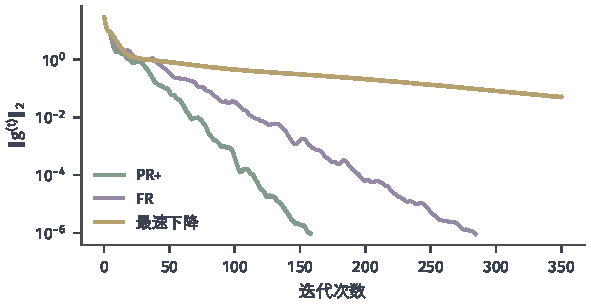
\includegraphics[width=100.0mm]{figures/05-optimization/06-constrained-optimization/matplotlib/mfo-rcg-compare/figure.pdf}
 \caption{$n=200$，$\bm{A}$的特征值在$1$到$100$之间等距，随机起点固定，球面上沿拉回函数作精确线搜索，用投影搬运。绿、紫分别为PR+与FR，黄色为最速下降。纵轴是黎曼梯度范数，最速下降在$350$轮内远未达到容差。}
 \label{fig:mfo-rcg-compare}
\end{BookInlineFigure}

\paragraph{需要核对的条件}
欧氏共轭梯度的保证不能直接照搬，有四项需要逐一核对。第一是方向的下降性。对式~\eqref{eq:mfo-rcg-direction}与$\bm{g}^{(t+1)}$作内积，得到
\[
 \langle\bm{g}^{(t+1)},\bm{d}^{(t+1)}\rangle=-\lVert\bm{g}^{(t+1)}\rVert_2^2+\beta^{(t+1)}\langle\bm{g}^{(t+1)},\mathcal{T}(\bm{d}^{(t)})\rangle.
\]
右端第二项若为正且较大，方向就不是下降方向。

第二是线搜索与搬运是否配套。欧氏情形下强Wolfe条件控制的正是$\langle\bm{g}^{(t+1)},\bm{d}^{(t)}\rangle$的大小。流形上线搜索控制的是一元函数的导数
\[
 \phi'(\alpha)=\bigl\langle\bm{g}^{(t+1)},\mathcal{T}^{\mathrm{D}}_{\alpha\bm{d}}(\bm{d})\bigr\rangle,
\]
它使用的是微分回缩。若方向更新用了另一种搬运，线搜索就控制不到上式第二项。

球面归一化时这个问题比较简单：第~\ref{sec:mfo-transport}节已指出投影搬运只差一个正因子$r$。例中$\langle\bm{g}^{(1)},\widetilde{\bm{d}}\rangle\approx-0.1171$，而$r=\tfrac{7\sqrt2}{9}$，所以$\phi'(\tfrac12)\approx-0.1064$。这个配套关系是例子的特殊之处，一般不成立。

第三是搬运的范数。关于FR的全局收敛分析通常要求搬运后的方向不比原方向长，否则可以用一个缩放因子修正。投影搬运满足这一点，平行移动也满足。证明需要把Zoutendijk型的求和论证搬到流形上，篇幅较长，读者可查阅关于黎曼共轭梯度收敛的专门文献。其结论大意是：强Wolfe条件和不增长的搬运使FR方向保持下降，并且$\liminf_{t\to\infty}\lVert\bm{g}^{(t)}\rVert_2=0$。

第四是重启。一方面下降性检查失败时需要重启；另一方面在非二次目标上旧方向会过时，常用的做法是每隔$\dim M$轮或连续两轮梯度明显不正交时重启。FR、PR+、搬运、线搜索的组合不同，保证也不同，任意组合不能默认继承欧氏结论。
